%%%%%%%%%%%%%%%%%%%%%%%%%%%%%%%%%%%%%%%%%%%%%%%%%%%%%%%%%%%%%%%%%%%%%%%%%%%%%%%%%%%%%%%%%%%%%%%%%
%
% Document:     Data Management  product tree
%
%%%%%%%%%%%%%%%%%%%%%%%%%%%%%%%%%%%%%%%%%%%%%%%%%%%%%%%%%%%%%%%%%%%%%%%%%%%%%%
\documentclass{article}
\usepackage{times,layouts}
\usepackage{tikz,hyperref,amsmath}
\usetikzlibrary{positioning,arrows,shapes,decorations.shapes,shapes.arrows}
\usetikzlibrary{backgrounds,calc}
\usepackage[paperwidth=1221.9999999999998pt,paperheight=731pt,
left=-2mm,top=3mm,bottom=0mm,right=0mm,
noheadfoot,marginparwidth=0pt,includemp=false,
textwidth=30cm,textheight=50mm]{geometry}
\newcommand\showpage{%
\setlayoutscale{0.5}\setlabelfont{\tiny}\printheadingsfalse\printparametersfalse
\currentpage\pagedesign}
\hypersetup{pdftitle={Data Management products }, pdfsubject={Diagram illustrating the
                products in LSST Data Management }, pdfauthor={Extracted from MagicDraw}}
\tikzstyle{tbox}=[rectangle,text centered, text width=30mm]
\tikzstyle{wbbox}=[rectangle, rounded corners=3pt, draw=black, top color=blue!50!white,
                    bottom color=white, very thick, minimum height=40pt, inner sep=2pt,
                    text centered, text width=30mm]
\tikzstyle{pbox}=[rectangle, rounded corners=3pt, draw=black, top
 color=yellow!50!white, bottom color=white, very thick,
 minimum height=36pt, inner sep=3pt, text centered, text width=35mm]
\tikzstyle{pline}=[-, thick]
\begin{document}
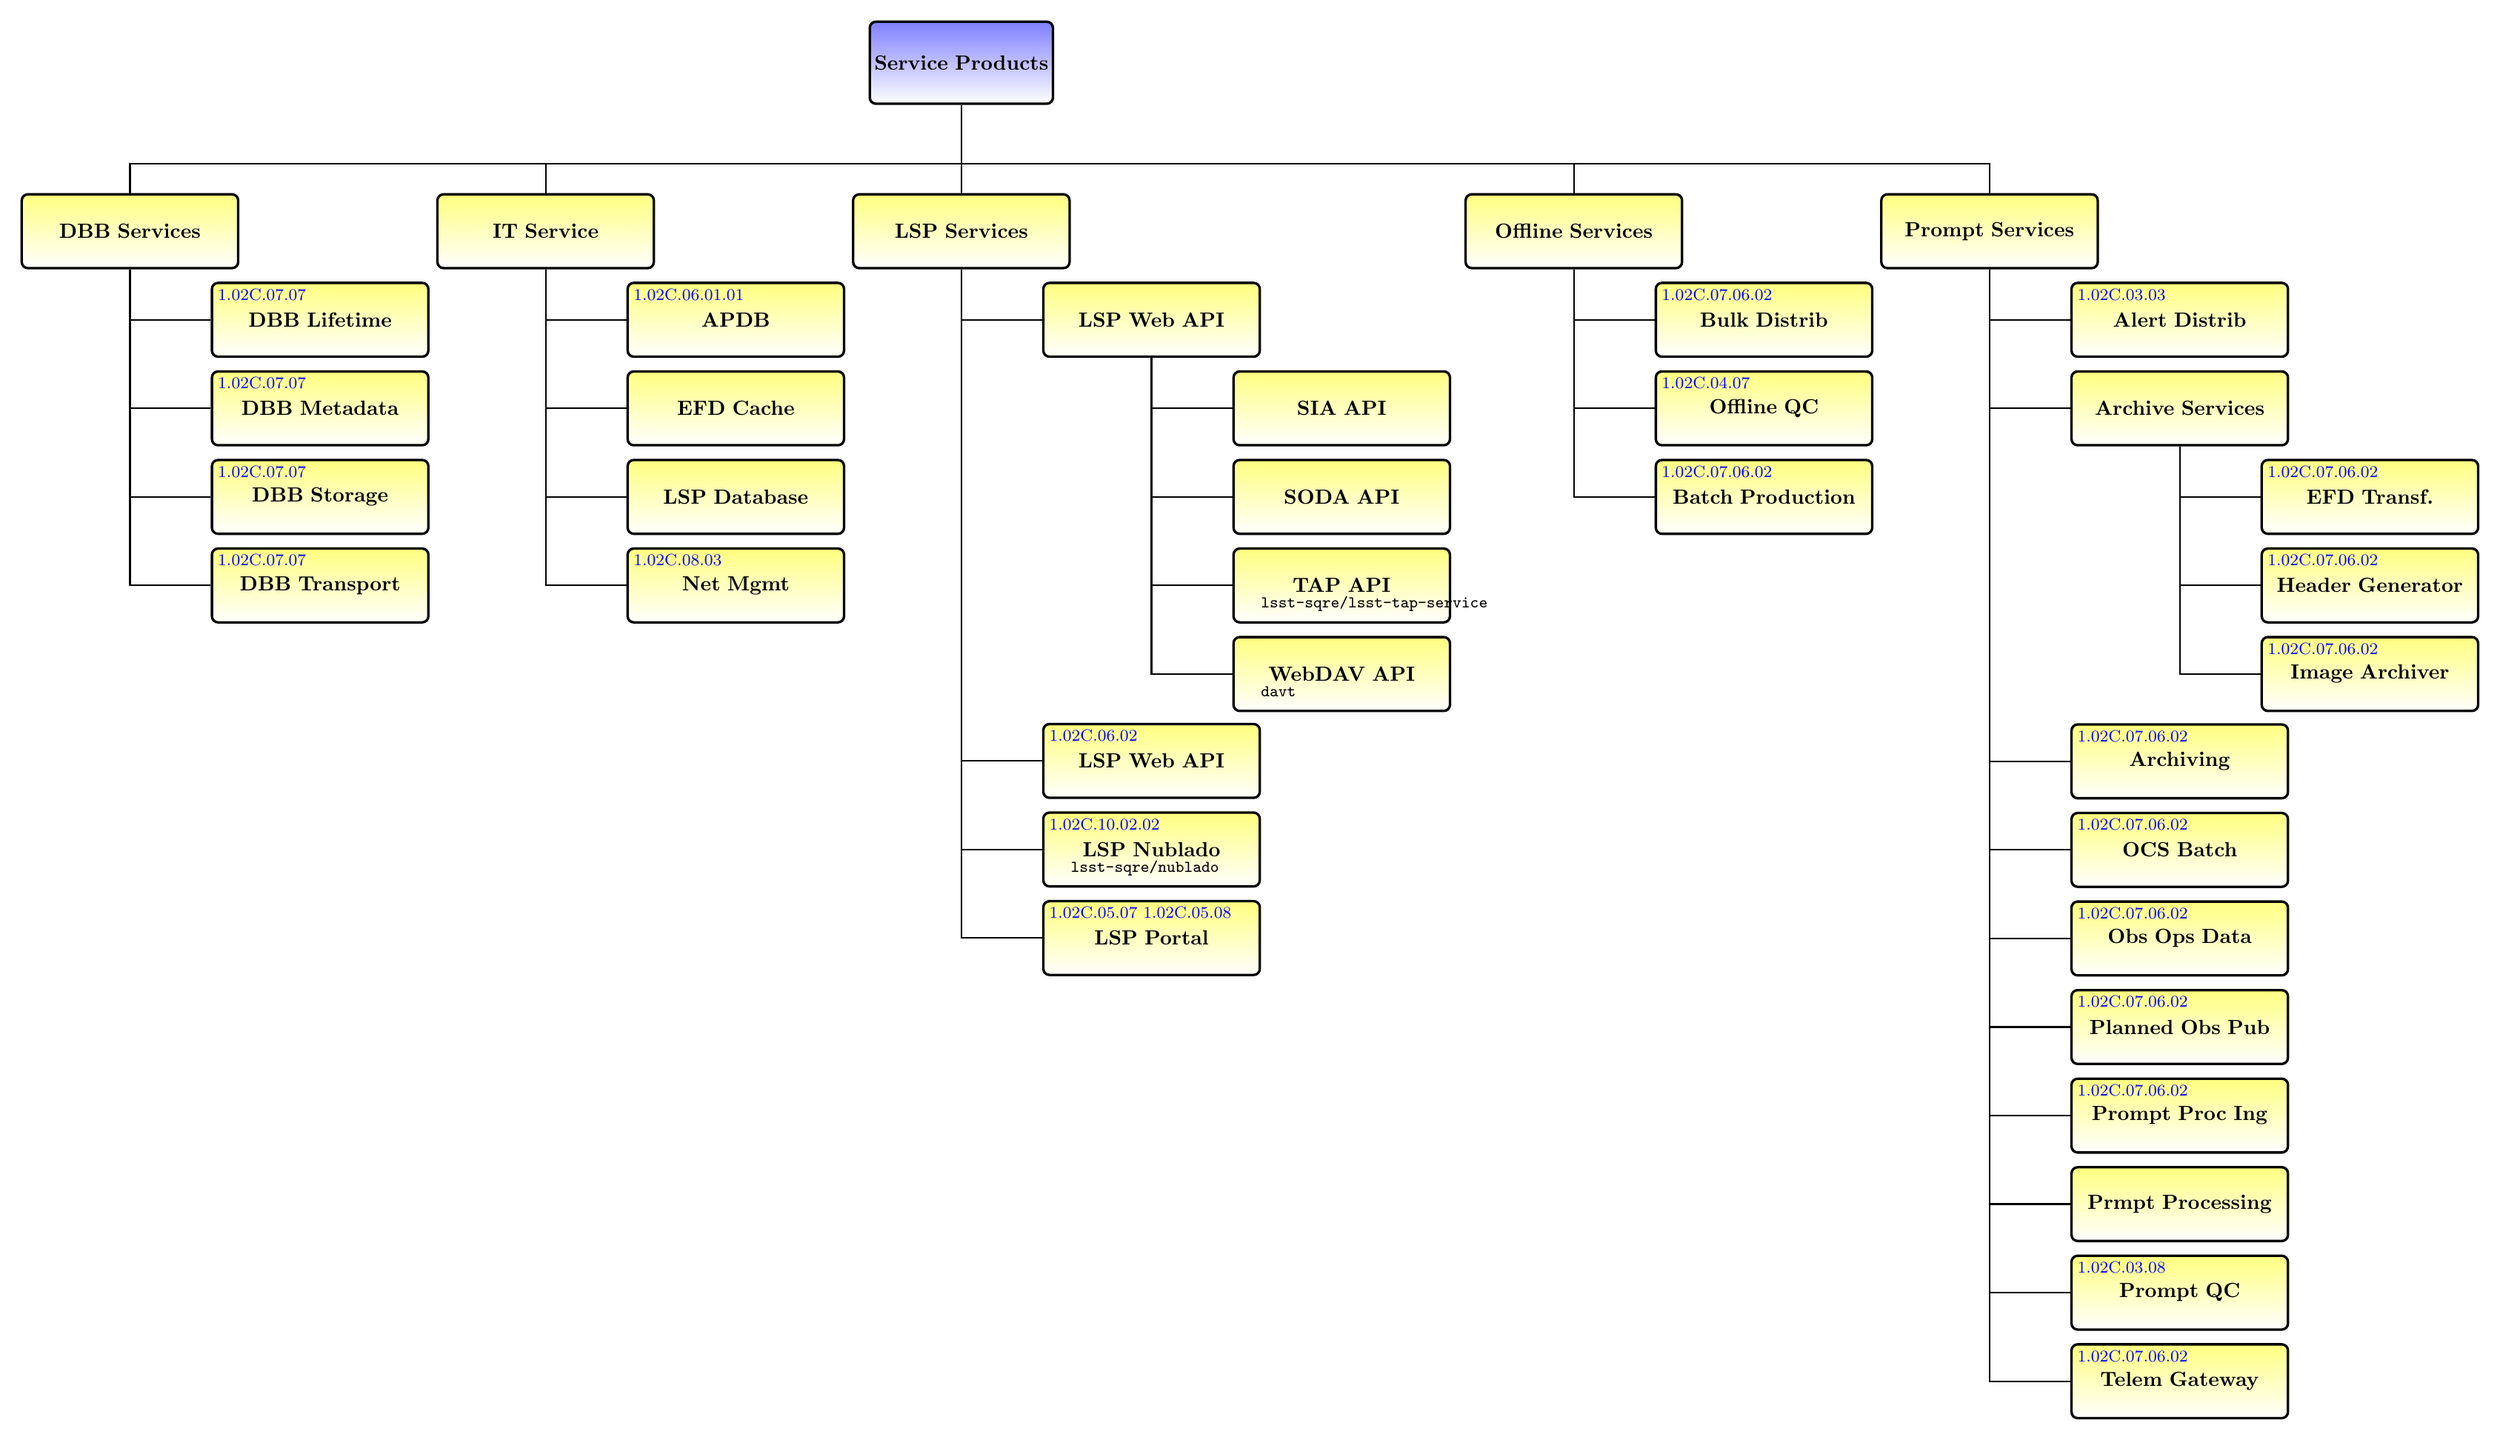
\begin{tikzpicture}[node distance=0mm]


\node (DBBSRV) [pbox, 
] {\textbf{DBB Services
} };\node [below right] at (DBBSRV.north west) {\footnotesize \color{blue}} ;

\node (DBBLIFESRV) [pbox,below right=6pt and -14pt of DBBSRV] {\textbf{DBB Lifetime
} };\node [below right] at (DBBLIFESRV.north west) {\footnotesize \color{blue}1.02C.07.07} ;

 \draw[pline] (DBBSRV.south) -| ++(0,0) |- (DBBLIFESRV.west); 
\node (DBBMDSRV) [pbox,below=6pt of DBBLIFESRV] {\textbf{DBB Metadata
} };\node [below right] at (DBBMDSRV.north west) {\footnotesize \color{blue}1.02C.07.07} ;

 \draw[pline] (DBBSRV.south) -| ++(0,0) |- (DBBMDSRV.west); 
\node (DBBSTRSRV) [pbox,below=6pt of DBBMDSRV] {\textbf{DBB Storage
} };\node [below right] at (DBBSTRSRV.north west) {\footnotesize \color{blue}1.02C.07.07} ;

 \draw[pline] (DBBSRV.south) -| ++(0,0) |- (DBBSTRSRV.west); 
\node (DBBTRSRV) [pbox,below=6pt of DBBSTRSRV] {\textbf{DBB Transport
} };\node [below right] at (DBBTRSRV.north west) {\footnotesize \color{blue}1.02C.07.07} ;

 \draw[pline] (DBBSRV.south) -| ++(0,0) |- (DBBTRSRV.west); 
\node (ITSRV) [pbox, 
right=96pt of DBBSRV] {\textbf{IT Service
} };\node [below right] at (ITSRV.north west) {\footnotesize \color{blue}} ;

\node (APDB) [pbox,below right=6pt and -14pt of ITSRV] {\textbf{APDB
} };\node [below right] at (APDB.north west) {\footnotesize \color{blue}1.02C.06.01.01} ;

 \draw[pline] (ITSRV.south) -| ++(0,0) |- (APDB.west); 
\node (EFDB) [pbox,below=6pt of APDB] {\textbf{EFD Cache
} };\node [below right] at (EFDB.north west) {\footnotesize \color{blue}} ;

 \draw[pline] (ITSRV.south) -| ++(0,0) |- (EFDB.west); 
\node (LSPDB) [pbox,below=6pt of EFDB] {\textbf{LSP Database
} };\node [below right] at (LSPDB.north west) {\footnotesize \color{blue}} ;

 \draw[pline] (ITSRV.south) -| ++(0,0) |- (LSPDB.west); 
\node (NETMGMT) [pbox,below=6pt of LSPDB] {\textbf{Net Mgmt
} };\node [below right] at (NETMGMT.north west) {\footnotesize \color{blue}1.02C.08.03} ;

 \draw[pline] (ITSRV.south) -| ++(0,0) |- (NETMGMT.west); 
\node (LSPSRV) [pbox, 
right=96pt of ITSRV] {\textbf{LSP Services
} };\node [below right] at (LSPSRV.north west) {\footnotesize \color{blue}} ;

\node (LSPWAPI) [pbox,below right=6pt and -14pt of LSPSRV] {\textbf{LSP Web API
} };\node [below right] at (LSPWAPI.north west) {\footnotesize \color{blue}} ;

 \draw[pline] (LSPSRV.south) -| ++(0,0) |- (LSPWAPI.west); 
\node (SIASRV) [pbox,below right=6pt and -14pt of LSPWAPI] {\textbf{SIA API
} };\node [below right] at (SIASRV.north west) {\footnotesize \color{blue}} ;

 \draw[pline] (LSPWAPI.south) -| ++(0,0) |- (SIASRV.west); 
\node (SODASRV) [pbox,below=6pt of SIASRV] {\textbf{SODA API
} };\node [below right] at (SODASRV.north west) {\footnotesize \color{blue}} ;

 \draw[pline] (LSPWAPI.south) -| ++(0,0) |- (SODASRV.west); 
\node (TAPSRV) [pbox,below=6pt of SODASRV] {\textbf{TAP API
} };\node [below right] at (TAPSRV.north west) {\footnotesize \color{blue}} ;
\node (TAPSRVpkg) [tbox,below=3mm of TAPSRV.north] {{\footnotesize \color{black} \begin{verbatim} lsst-sqre/lsst-tap-service \end{verbatim} }  };

 \draw[pline] (LSPWAPI.south) -| ++(0,0) |- (TAPSRV.west); 
\node (WDAVSRV) [pbox,below=6pt of TAPSRV] {\textbf{WebDAV API
} };\node [below right] at (WDAVSRV.north west) {\footnotesize \color{blue}} ;
\node (WDAVSRVpkg) [tbox,below=3mm of WDAVSRV.north] {{\footnotesize \color{black} \begin{verbatim} davt \end{verbatim} }  };

 \draw[pline] (LSPWAPI.south) -| ++(0,0) |- (WDAVSRV.west); 
\node (LSPWEBSRV) [pbox,below=178pt of LSPWAPI] {\textbf{LSP Web API
} };\node [below right] at (LSPWEBSRV.north west) {\footnotesize \color{blue}1.02C.06.02} ;

 \draw[pline] (LSPSRV.south) -| ++(0,0) |- (LSPWEBSRV.west); 
\node (NBLSRV) [pbox,below=6pt of LSPWEBSRV] {\textbf{LSP Nublado
} };\node [below right] at (NBLSRV.north west) {\footnotesize \color{blue}1.02C.10.02.02} ;
\node (NBLSRVpkg) [tbox,below=3mm of NBLSRV.north] {{\footnotesize \color{black} \begin{verbatim} lsst-sqre/nublado \end{verbatim} }  };

 \draw[pline] (LSPSRV.south) -| ++(0,0) |- (NBLSRV.west); 
\node (PRTLSRV) [pbox,below=6pt of NBLSRV] {\textbf{LSP Portal
} };\node [below right] at (PRTLSRV.north west) {\footnotesize \color{blue}1.02C.05.07 1.02C.05.08} ;

 \draw[pline] (LSPSRV.south) -| ++(0,0) |- (PRTLSRV.west); 
\node (OFFLSRV) [pbox, 
right=192pt of LSPSRV] {\textbf{Offline Services
} };\node [below right] at (OFFLSRV.north west) {\footnotesize \color{blue}} ;

\node (BULKDSRV) [pbox,below right=6pt and -14pt of OFFLSRV] {\textbf{Bulk Distrib
} };\node [below right] at (BULKDSRV.north west) {\footnotesize \color{blue}1.02C.07.06.02} ;

 \draw[pline] (OFFLSRV.south) -| ++(0,0) |- (BULKDSRV.west); 
\node (OFFLQCSRV) [pbox,below=6pt of BULKDSRV] {\textbf{Offline QC
} };\node [below right] at (OFFLQCSRV.north west) {\footnotesize \color{blue}1.02C.04.07} ;

 \draw[pline] (OFFLSRV.south) -| ++(0,0) |- (OFFLQCSRV.west); 
\node (PRODSRV) [pbox,below=6pt of OFFLQCSRV] {\textbf{Batch Production
} };\node [below right] at (PRODSRV.north west) {\footnotesize \color{blue}1.02C.07.06.02} ;

 \draw[pline] (OFFLSRV.south) -| ++(0,0) |- (PRODSRV.west); 
\node (PRSRV) [pbox, 
right=96pt of OFFLSRV] {\textbf{Prompt Services
} };\node [below right] at (PRSRV.north west) {\footnotesize \color{blue}} ;

\node (ALRTDSTSRV) [pbox,below right=6pt and -14pt of PRSRV] {\textbf{Alert Distrib
} };\node [below right] at (ALRTDSTSRV.north west) {\footnotesize \color{blue}1.02C.03.03} ;

 \draw[pline] (PRSRV.south) -| ++(0,0) |- (ALRTDSTSRV.west); 
\node (ARCSRVS) [pbox,below=6pt of ALRTDSTSRV] {\textbf{Archive Services
} };\node [below right] at (ARCSRVS.north west) {\footnotesize \color{blue}} ;

 \draw[pline] (PRSRV.south) -| ++(0,0) |- (ARCSRVS.west); 
\node (EFDTS) [pbox,below right=6pt and -14pt of ARCSRVS] {\textbf{EFD Transf.
} };\node [below right] at (EFDTS.north west) {\footnotesize \color{blue}1.02C.07.06.02} ;

 \draw[pline] (ARCSRVS.south) -| ++(0,0) |- (EFDTS.west); 
\node (HEADS) [pbox,below=6pt of EFDTS] {\textbf{Header Generator
} };\node [below right] at (HEADS.north west) {\footnotesize \color{blue}1.02C.07.06.02} ;

 \draw[pline] (ARCSRVS.south) -| ++(0,0) |- (HEADS.west); 
\node (IMAS) [pbox,below=6pt of HEADS] {\textbf{Image Archiver
} };\node [below right] at (IMAS.north west) {\footnotesize \color{blue}1.02C.07.06.02} ;

 \draw[pline] (ARCSRVS.south) -| ++(0,0) |- (IMAS.west); 
\node (ARCSRVo) [pbox,below=135pt of ARCSRVS] {\textbf{Archiving
} };\node [below right] at (ARCSRVo.north west) {\footnotesize \color{blue}1.02C.07.06.02} ;

 \draw[pline] (PRSRV.south) -| ++(0,0) |- (ARCSRVo.west); 
\node (OCSBATSRV) [pbox,below=6pt of ARCSRVo] {\textbf{OCS Batch
} };\node [below right] at (OCSBATSRV.north west) {\footnotesize \color{blue}1.02C.07.06.02} ;

 \draw[pline] (PRSRV.south) -| ++(0,0) |- (OCSBATSRV.west); 
\node (OODSSRV) [pbox,below=6pt of OCSBATSRV] {\textbf{Obs Ops Data
} };\node [below right] at (OODSSRV.north west) {\footnotesize \color{blue}1.02C.07.06.02} ;

 \draw[pline] (PRSRV.south) -| ++(0,0) |- (OODSSRV.west); 
\node (POPSRV) [pbox,below=6pt of OODSSRV] {\textbf{Planned Obs Pub
} };\node [below right] at (POPSRV.north west) {\footnotesize \color{blue}1.02C.07.06.02} ;

 \draw[pline] (PRSRV.south) -| ++(0,0) |- (POPSRV.west); 
\node (PRPINGSRV) [pbox,below=6pt of POPSRV] {\textbf{Prompt Proc Ing
} };\node [below right] at (PRPINGSRV.north west) {\footnotesize \color{blue}1.02C.07.06.02} ;

 \draw[pline] (PRSRV.south) -| ++(0,0) |- (PRPINGSRV.west); 
\node (PRPRSRV) [pbox,below=6pt of PRPINGSRV] {\textbf{Prmpt Processing
} };\node [below right] at (PRPRSRV.north west) {\footnotesize \color{blue}} ;

 \draw[pline] (PRSRV.south) -| ++(0,0) |- (PRPRSRV.west); 
\node (PRQCSRV) [pbox,below=6pt of PRPRSRV] {\textbf{Prompt QC
} };\node [below right] at (PRQCSRV.north west) {\footnotesize \color{blue}1.02C.03.08} ;

 \draw[pline] (PRSRV.south) -| ++(0,0) |- (PRQCSRV.west); 
\node (TMGSRV) [pbox,below=6pt of PRQCSRV] {\textbf{Telem Gateway
} };\node [below right] at (TMGSRV.north west) {\footnotesize \color{blue}1.02C.07.06.02} ;

 \draw[pline] (PRSRV.south) -| ++(0,0) |- (TMGSRV.west); 
\node (DMSRV) [wbbox, above=43pt of LSPSRV]{\textbf{Service Products}};
 \draw[pline]   (DBBSRV.north) -- ++(0.0,0.5) -| (DMSRV.south) ; 
 \draw[pline]   (ITSRV.north) -- ++(0.0,0.5) -| (DMSRV.south) ; 
 \draw[pline]   (LSPSRV.north) -- ++(0.0,0.5) -| (DMSRV.south) ; 
 \draw[pline]   (OFFLSRV.north) -- ++(0.0,0.5) -| (DMSRV.south) ; 
 \draw[pline]   (PRSRV.north) -- ++(0.0,0.5) -| (DMSRV.south) ; 

\end{tikzpicture}
\end{document}
